\hypertarget{test__replace2_8cpp}{}\subsection{test\+\_\+replace2.\+cpp File Reference}
\label{test__replace2_8cpp}\index{test\+\_\+replace2.\+cpp@{test\+\_\+replace2.\+cpp}}


Contains an example to take subject string, replacement string, modifier and pattern from user input and perform regex replace with J\+P\+C\+R\+E2.  


{\ttfamily \#include $<$iostream$>$}\newline
{\ttfamily \#include \char`\"{}jpcre2.\+hpp\char`\"{}}\newline
Include dependency graph for test\+\_\+replace2.\+cpp\+:\nopagebreak
\begin{figure}[H]
\begin{center}
\leavevmode
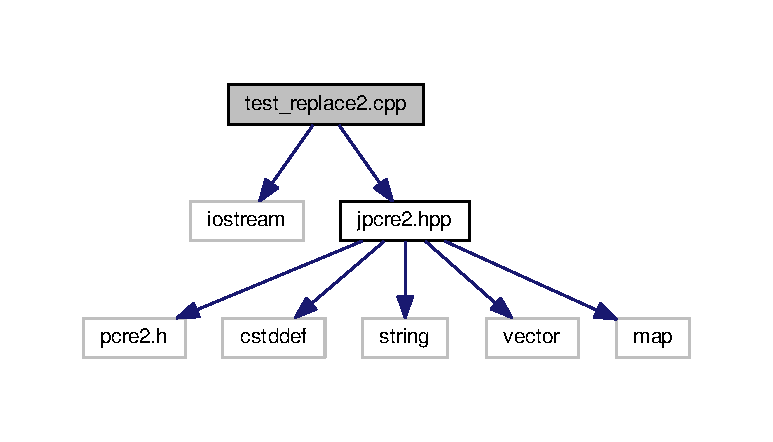
\includegraphics[width=350pt]{test__replace2_8cpp__incl}
\end{center}
\end{figure}


\subsubsection{Detailed Description}
Contains an example to take subject string, replacement string, modifier and pattern from user input and perform regex replace with J\+P\+C\+R\+E2. 


\begin{DoxyCodeInclude}

\textcolor{preprocessor}{#include <iostream>}
\textcolor{preprocessor}{#include "\hyperlink{jpcre2_8hpp}{jpcre2.hpp}"}


\textcolor{preprocessor}{#define getLine(a) std::getline(std::cin,a,'\(\backslash\)n')}


\textcolor{keywordtype}{int} main()\{
    std::string pat,mod,subject,repl,repl\_mod;

    std::cout<<\textcolor{stringliteral}{"\(\backslash\)nEnter pattern: "};
    getLine(pat);

    std::cout<<\textcolor{stringliteral}{"\(\backslash\)nEnter compile modifiers (eijmnsuxADJSU): "};
    getLine(mod);
    \hyperlink{classjpcre2_1_1Regex}{jpcre2::Regex} re;     \textcolor{comment}{// This is not supposed to throw any exception.}


    \textcolor{comment}{// Compile the pattern}
    \textcolor{keywordflow}{try}\{re.\hyperlink{classjpcre2_1_1Regex_aad1d5ef1e87f762f68a587eec4022e69_aad1d5ef1e87f762f68a587eec4022e69}{compile}(pat,mod);\}
    \textcolor{keywordflow}{catch}(\hyperlink{classjpcre2_1_1Except}{jpcre2::Except}& e)\{std::cerr<<e.\hyperlink{classjpcre2_1_1Except_a6781e0804575f11d6d8bb87ec2d036c6_a6781e0804575f11d6d8bb87ec2d036c6}{getErrorMessage}();\}


    \textcolor{comment}{/******************************************************************************************************
      *********}
\textcolor{comment}{     * All jpcre2 exceptions are of type jpcre2::Except}
\textcolor{comment}{     * ****************************************************************************************************
      *********/}


    \textcolor{comment}{// subject string}
    std::cout<<\textcolor{stringliteral}{"\(\backslash\)nEnter subject string (enter quit to quit): "}<<std::endl;
    getLine(subject);
    \textcolor{keywordflow}{if}(subject==\textcolor{stringliteral}{"quit"})\textcolor{keywordflow}{return} 0;
     \textcolor{comment}{//replacement string}
    std::cout<<\textcolor{stringliteral}{"\(\backslash\)nEnter replacement string: "}<<std::endl;
    getLine(repl);

    \textcolor{comment}{// Continue loop as long as error occurs}
    \textcolor{keywordflow}{while}(\textcolor{keyword}{true})\{
        std::cout<<\textcolor{stringliteral}{"\(\backslash\)nEnter action (replacement) modifiers (eEgx): "};
        getLine(repl\_mod);

        \textcolor{comment}{//perform replace}

        \textcolor{keywordflow}{try}\{std::cout<<\textcolor{stringliteral}{"\(\backslash\)nreplaced string: "}<<re.\hyperlink{classjpcre2_1_1Regex_ae7235a991492fa88f1bd3fb02d59cd0a_ae7235a991492fa88f1bd3fb02d59cd0a}{initReplace}()
                                                .\hyperlink{classjpcre2_1_1RegexReplace_a46eefdb105827920bebc8436721fa4cb_a46eefdb105827920bebc8436721fa4cb}{setSubject}(subject)
                                                .\hyperlink{classjpcre2_1_1RegexReplace_af1069f489de9b343493da2dc77b04c73_af1069f489de9b343493da2dc77b04c73}{setReplaceWith}(repl)
                                                .\hyperlink{classjpcre2_1_1RegexReplace_a3f86b1e11d08d0153a08244771e59061_a3f86b1e11d08d0153a08244771e59061}{addJpcre2Option}(
      \hyperlink{namespacejpcre2_a85c143271501e383843f45b9999c2f00_a85c143271501e383843f45b9999c2f00a9124b768bcae4d51430aa7f26126f387}{jpcre2::VALIDATE\_MODIFIER})
                                                .\hyperlink{classjpcre2_1_1RegexReplace_a06a57430f62058822d48722a2a6425d7_a06a57430f62058822d48722a2a6425d7}{addModifier}(repl\_mod)
                                                .\hyperlink{classjpcre2_1_1RegexReplace_afd087fa7a9bfedec802d1a3dd7edbdd0_afd087fa7a9bfedec802d1a3dd7edbdd0}{replace}();\}
        \textcolor{keywordflow}{catch}(\hyperlink{classjpcre2_1_1Except}{jpcre2::Except}& e)\{std::cerr<<e.\hyperlink{classjpcre2_1_1Except_a6781e0804575f11d6d8bb87ec2d036c6_a6781e0804575f11d6d8bb87ec2d036c6}{getErrorMessage}();
            \textcolor{keywordflow}{if}(e.\hyperlink{classjpcre2_1_1Except_a0f3e00116ab24b89836a2c2a66262e22_a0f3e00116ab24b89836a2c2a66262e22}{getErrorNumber}()==\hyperlink{namespacejpcre2_1_1ERROR_a4b2998984439438fa9da8d7043909bc2_a4b2998984439438fa9da8d7043909bc2a4115340549b623f4e2da285bf0aa9bff}{jpcre2::ERROR::INVALID\_MODIFIER}
      ) \textcolor{keywordflow}{continue};
        \}
        \textcolor{keywordflow}{break};
    \}
    std::cout<<\textcolor{stringliteral}{"\(\backslash\)n\(\backslash\)n--------------------------------------------------\(\backslash\)n"};

    \textcolor{keywordflow}{return} 0;
\}
\end{DoxyCodeInclude}
 \begin{DoxyAuthor}{Author}
\href{https://github.com/neurobin}{\tt Md Jahidul Hamid} 
\end{DoxyAuthor}
